\section{Gestione scenario}
	Per quanto riguarda la gestione degli \mglo{Scenario}{scenario} l'utente ha la possibilità di:
	\begin{itemize}
		\item aggiungere uno scenario;
		\item visualizzare i dettagli relativi a un certo scenario presente;
		\item modificare uno scenario presente;
		\item eliminare uno scenario presente.
	\end{itemize}

\subsection{Aggiunta di uno scenario}
	Per aggiungere uno scenario si deve:
	\begin{itemize}
		\item cliccare sul pulsante "+" in basso a destra della mappa;
		\item selezionare la voce "Aggiungi scenario";
		\item disegnare il perimetro dello scenario sulla mappa. E' possibile apporre gli spigoli del perimetro cliccando direttamente sulla mappa. Il perimetro dello scenario deve essere correttamente chiuso, facendo coincidere l'ultimo spigolo del perimetro col primo;
		\item compilare i campi (tutti) rispettando i vincoli esposti nell'apposita appendice \nameref{Validazioni};
		\item cliccare sul pulsante "Salva", che verrà abilitato solo nel momento in cui tutte le operazioni sopra descritte sono state eseguite in maniera corretta.
	\end{itemize}
	
	\begin{figure}[H]
	\centering
	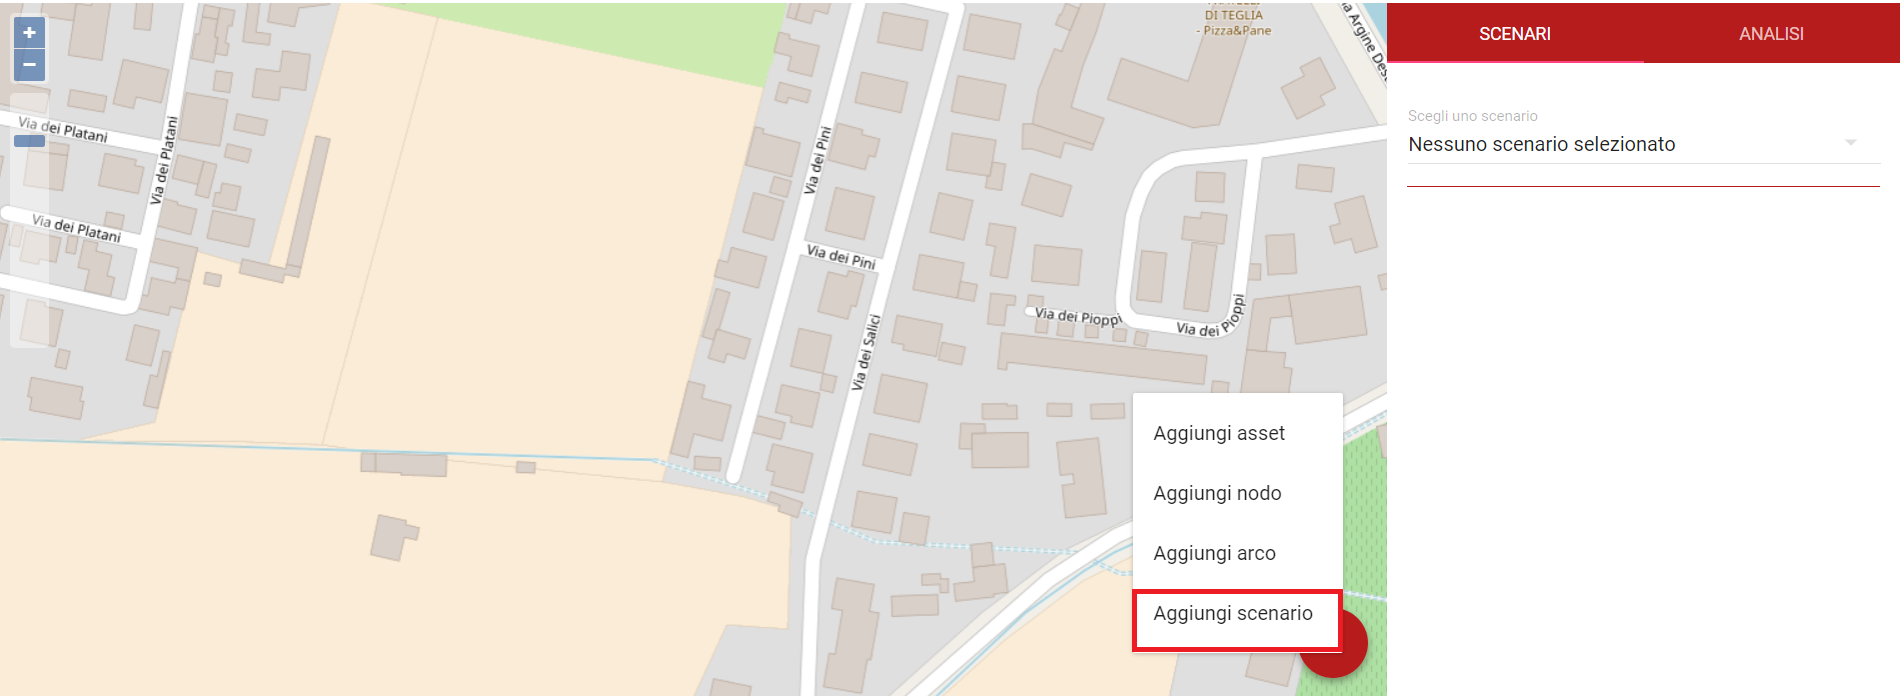
\includegraphics[width=\textwidth]{img/menu_aperto_scenario_hover.png}
	\caption{Menu di aggiunta}
	\end{figure}
	
	\begin{figure}[H]
	\centering
	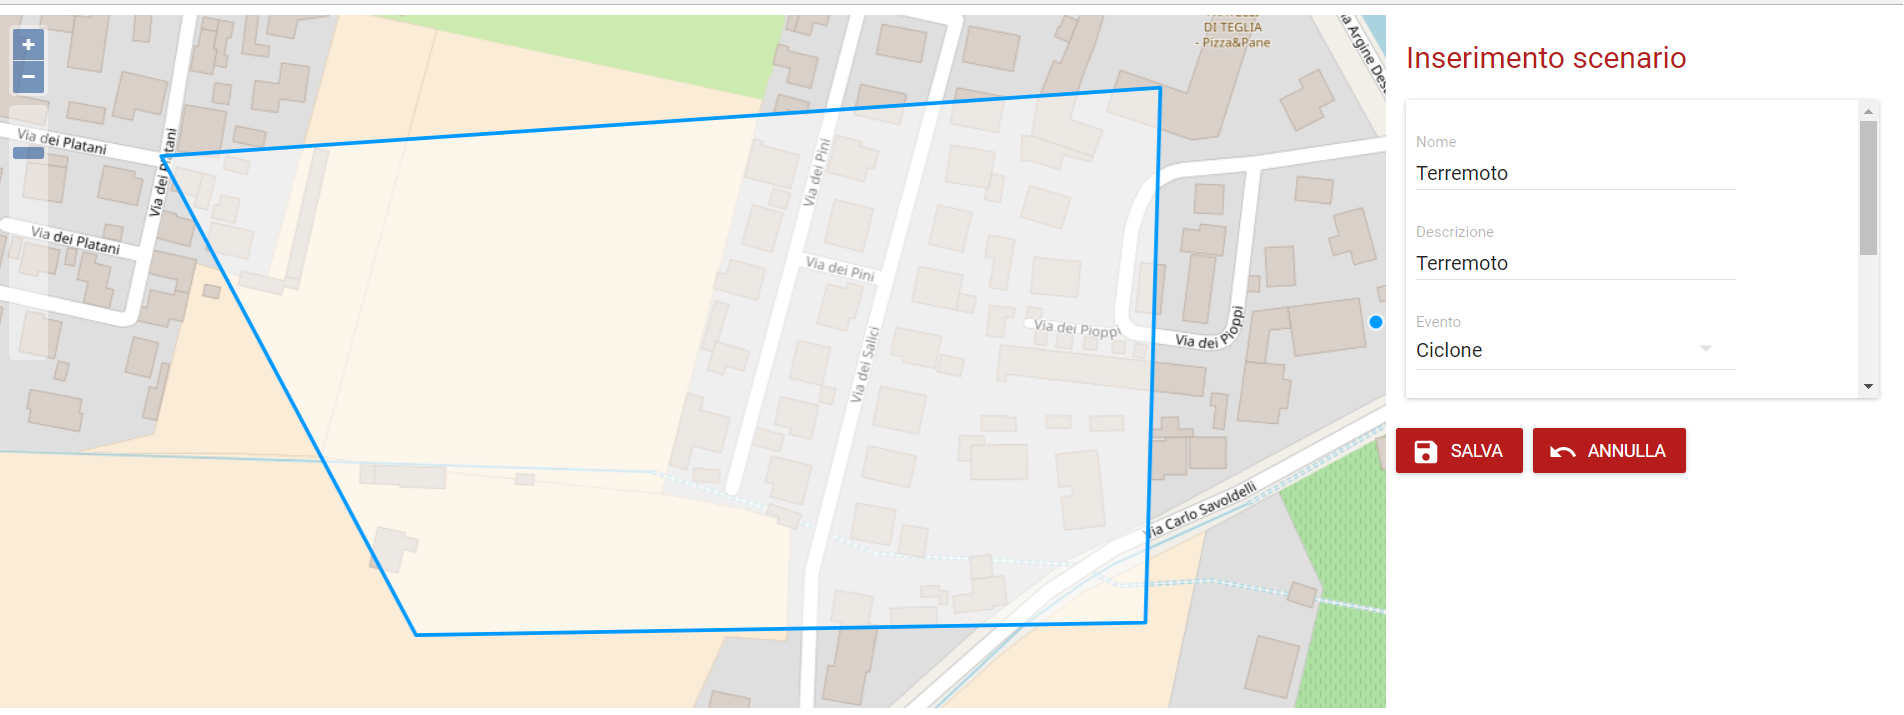
\includegraphics[width=\textwidth]{img/aggiunta_scenario.png}
	\caption{Aggiunta di uno scenario}
	\end{figure}

\subsection{Visualizzazione dei dettagli di uno scenario}
	Per visualizzare i dettagli di uno scenario si deve:
	\begin{itemize}
		\item selezionare l'scenario che si intende modificare cliccando direttamente su quell'scenario dalla mappa.
	\end{itemize}
	
	\begin{figure}[H]
	\centering
	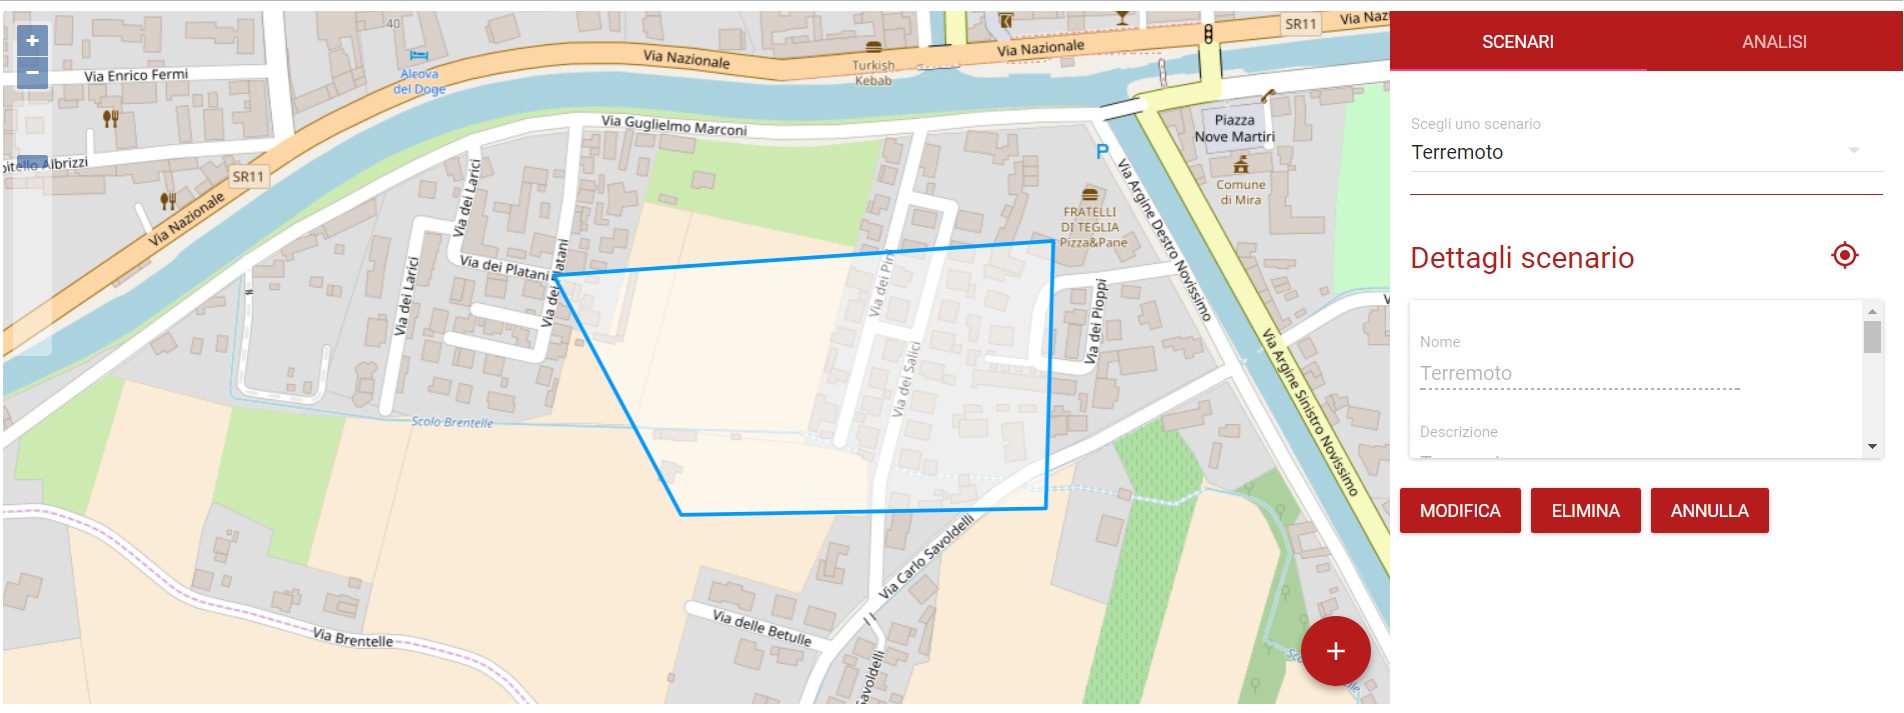
\includegraphics[width=\textwidth]{img/visualizzazione_scenario.png}
	\caption{Visualizzazione dettagli di uno scenario}
	\end{figure}

\subsection{Modifica di uno scenario}
	Per modificare uno scenario si deve:
	\begin{itemize}
		\item selezionare l'scenario che si intende modificare cliccando direttamente sulla mappa;
		\item cliccare sul pulsante "Modifica" in basso sulla sidebar;
		\item eventualmente ridisegnare il perimetro dello scenario sulla mappa. E' possibile apporre gli spigoli del perimetro cliccando direttamente sulla mappa. Il nuovo perimetro andrà in automatico a sovrascrivere quello precentemente presente. Il perimetro dello scenario deve essere correttamente chiuso, facendo coincidere l'ultimo spigolo del perimetro col primo;
		\item eventualmente modificare i campi rispettando i vincoli esposti nell'apposita appendice \nameref{Validazioni};
		\item cliccare sul pulsante "Salva", che verrà abilitato solo nel momento in cui tutte le operazioni sopra descritte sono state eseguite in maniera corretta.
	\end{itemize}
	
	\begin{figure}[H]
	\centering
	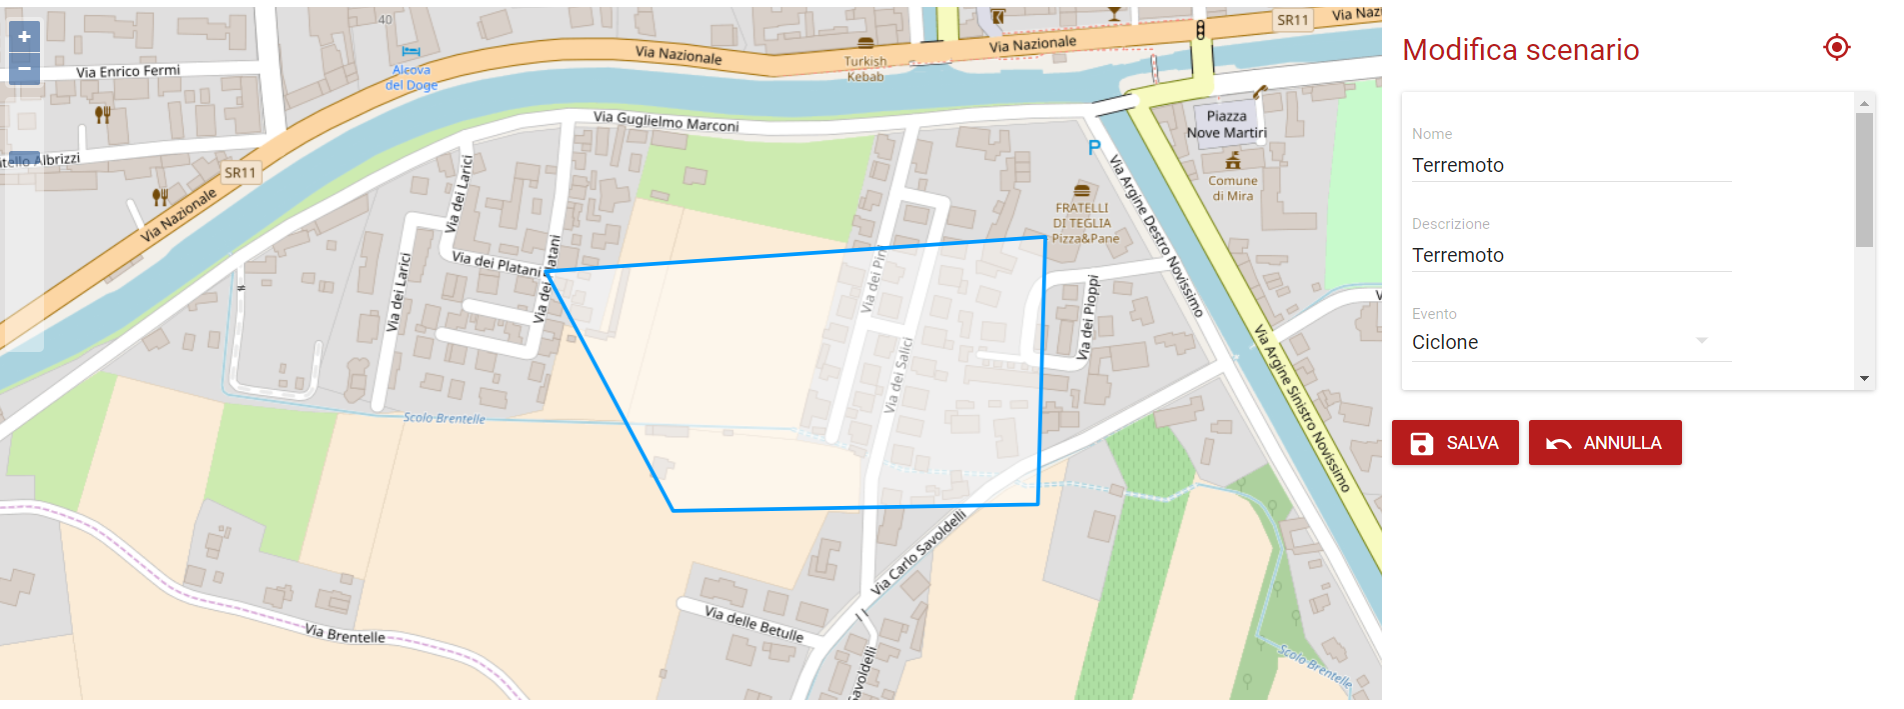
\includegraphics[width=\textwidth]{img/modifica_scenario.png}
	\caption{Modifica di uno scenario}
	\end{figure}

\subsection{Eliminazione di uno scenario}
Per eliminare uno scenario si deve:
\begin{itemize}
	\item selezionare l'scenario che si intende modificare cliccando direttamente sulla mappa;
	\item cliccare sul pulsante "Elimina" in basso sulla sidebar;
	\item cliccare sul pulsante "Elimina" sulla finestra bloccante che compare.
\end{itemize}

\begin{figure}[H]
\centering
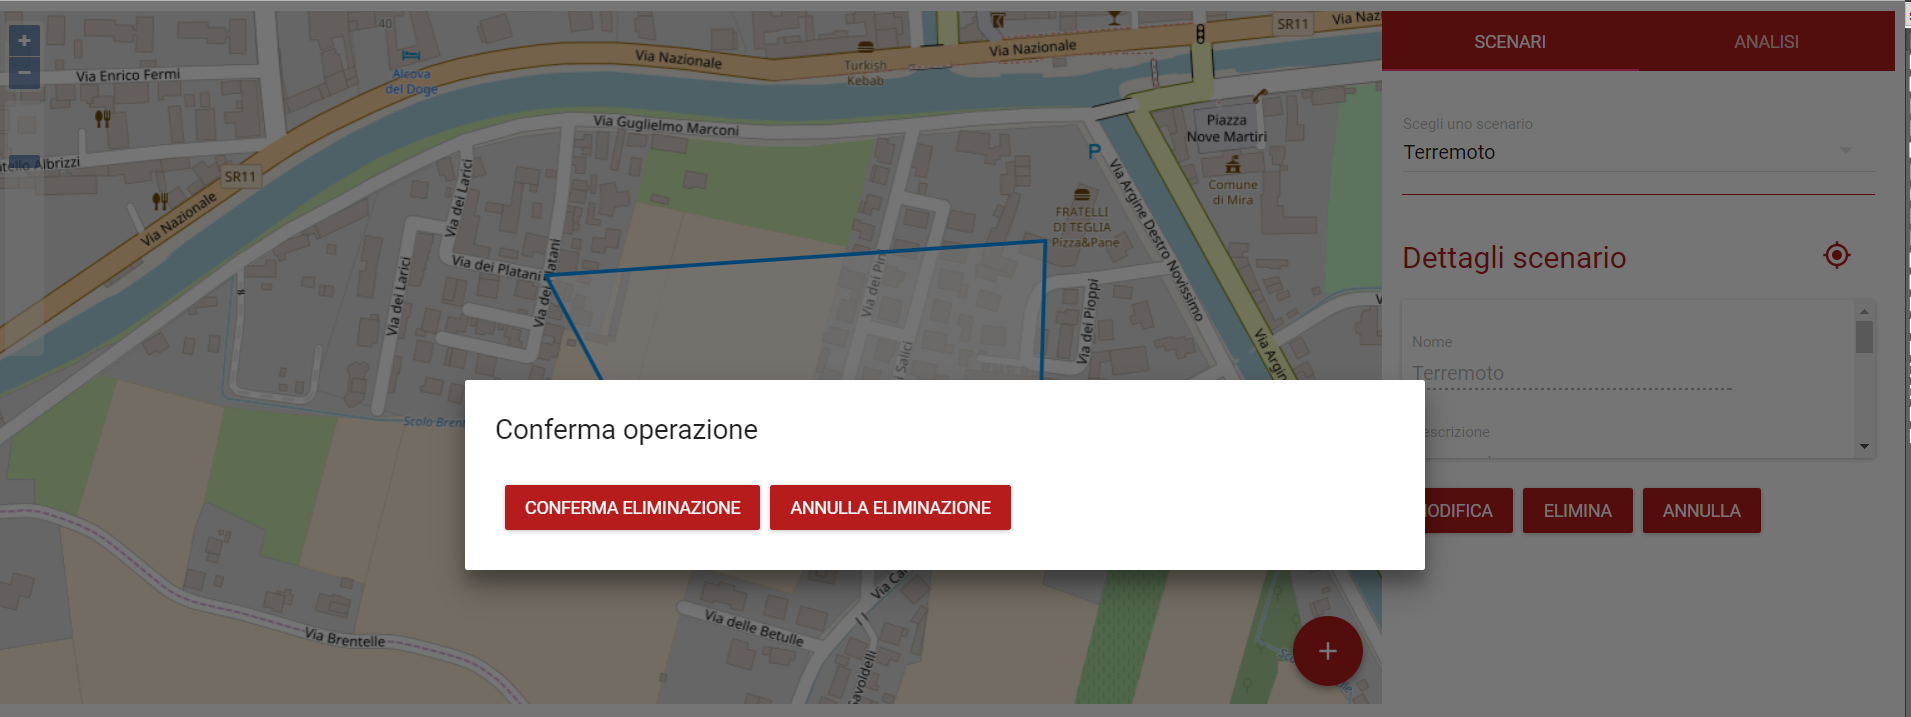
\includegraphics[width=\textwidth]{img/eliminazione_bloccante_scenario.png}
\caption{Eliminazione di uno scenario}
\end{figure}